\documentclass{beamer}
\usetheme{Gelugor}
\usepackage{hyperref}
\usepackage[utf8]{inputenc}
\usepackage[spanish]
\usepackage[default]{droidserif}
\usepackage{ragged2e}

\title{Análisis y Diseño de Sistemas}
\subtitle{Heroku | Cloud Application Platform.  Despliegue de aplicaciones a partir del GitHub}
\author{
Antonio Aguilar ECINF7224
Manuel Armijos ECINF7225 \\
Ricardo Jumbo ECINF7207 
Pablo Sarango ECINF7226 \\
Luís Solano AFINF7205
Jefferson Vera ECINF7434.
}
\date{\today}
\institute{Ingeniería en Sistemas\\}

\begin{document}
\justifying
	
	%INICIO carátula
	\begin{frame}[plain,t]
		\titlepage
	\end{frame}
	%FIN carátula

	\section{Tema}

	\subsection{Introducción}
		\begin{frame}
			\frametitle{Introducción}
			%\framesubtitle{Tema}
			A continuación se mostrará el despliegue de una aplicación sencilla a partir de GitHub. Para el despliegue se ha usado Heroku: Una Plataforma como Servicio (PaaS).\\ \ \\
			
			Es un servicio de Hosting en la nube(los clientes no tienen que contar con infraestructura, el tiempo de procesamiento y almacenamiento se le renta a un tercero).\\ \ \\
			
			Fue Fundada en 2007 y adquirida por Salesforce.com en 2011.
		\end{frame}
		
		\subsection{Características}
		\begin{frame}			
			\frametitle{Características}\\
			\begin{itemize}
			\item Servicio basados en la nube de Amazon Web Services(ECS,S3, etc.)
			\item La implementacion se hace a traves de Git.
			\item Gratuito(hasta 5 MB de espacio para base de datos, 50MB para todos los archivos incluyendo repositorios Git).
			\item En la aplicacion ”compilada” nos brinda un Máximo de 100MB.
			\end{itemize}
		\end{frame}	
		
		\subsection{Características}
		\begin{frame}
			\frametitle{Características}\\
			\begin{itemize}
			\item Esta basada en SO Debian y Ruby 1.8.X.
			\item Bajo costo para apps pequeñas.
			\item Ofrece manejo sencillo de apps complejas.
			\item La unidad básica de procesamiento son los Dynos, costo  0,05 USD por hora o 0,10 USD por hora.
			\end{itemize}
		\end{frame}
		
		\subsection{Clientes}
		\begin{frame}
			\frametitle{Clientes}
			\begin{itemize}
			\item GitHub.
			\item Code for America.
			\item TED.
			\item Facebook.
			\item MailChimp.
			\item Entre otros.
			\end{itemize}
		\end{frame}
			
			 
\end{frame}
\subsection{Agenda}
\begin{frame}
\frametitle{Agenda}
\begin{itemize}
\item Heroku
	\begin{itemize}
	\item Servicios en Heroku
	\item Importancia.
	\item Ventajas.
	\item Desventajas.
	\item Arquitectura.
	\item Registro
	\item Heroku Toolbelt
	\end{itemize}
\item Despliegue de aplicación
	\begin{itemize}
	\item GitHub
	\item Requisitos
	\item Despliegue en Heroku
	\end{itemize}
\item GitHub y Heroku
	\begin{itemize}
	\item Sincronización
	\item Commit en GitHub y Heroku.
	\item Despliegue automático.
	\item Despligue manual.
	\end{itemize}
\end{itemize}
\end{frame}

\subsection{Objetivos}
\begin{frame}
\frametitle{Objetivos}
%\begin{definition}[Greetings]
	\begin{itemize}
		\item Desplegar una aplicación a partir de GitHub en Heroku.
		\item Demostrar el uso de plataformas para el desarrollo colaborativo.
		\item Examinar el empleo Plataformas como Servicio o PaaS.
	\end{itemize}
%\end{definition}

%\begin{theorem}[Fermat's Last Theorem]
%$a^n + b^n = c^n, n \leq 2$
%\end{theorem}

%\begin{alertblock}{Uh-oh.}
%By the pricking of my thumbs.
%\end{alertblock}

%\begin{exampleblock}{Uh-oh.}
%Something evil this way comes.
%\end{exampleblock}

\end{frame}


\subsection{Desarrollo}
\begin{frame}
\frametitle{Heroku. Servicios}
Actualmente Heroku ofrece los siguiente servicios.\\ \ \\

\includegraphics[width=10cm, height=1cm]{ampliacion/1.png}
\end{frame}

\begin{frame}
\frametitle{Heroku. Servicios}
Base de datos.\\ \ \\
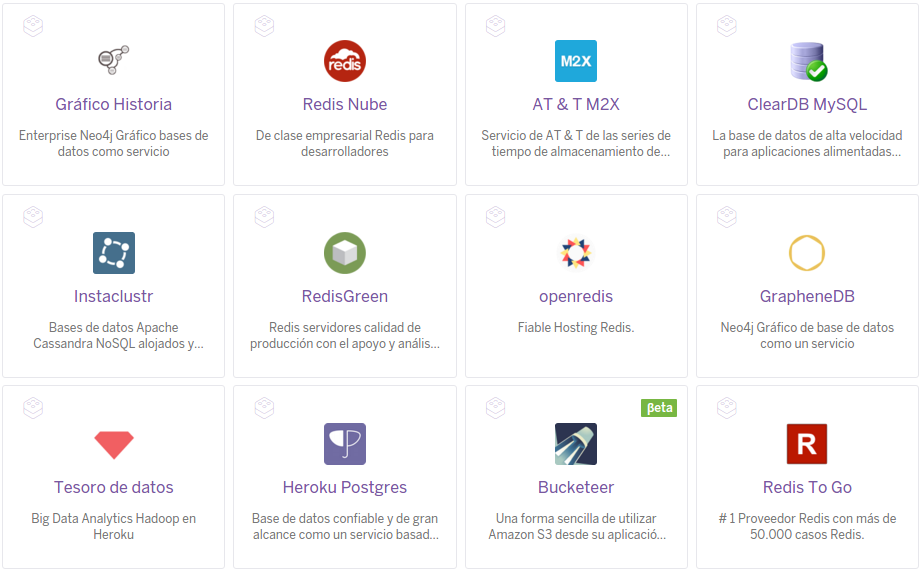
\includegraphics[width=10cm, height=5cm]{ampliacion/2.png}
\end{frame}

\begin{frame}
\frametitle{Heroku. Servicios}
Almacenes de datos.\\ \ \\
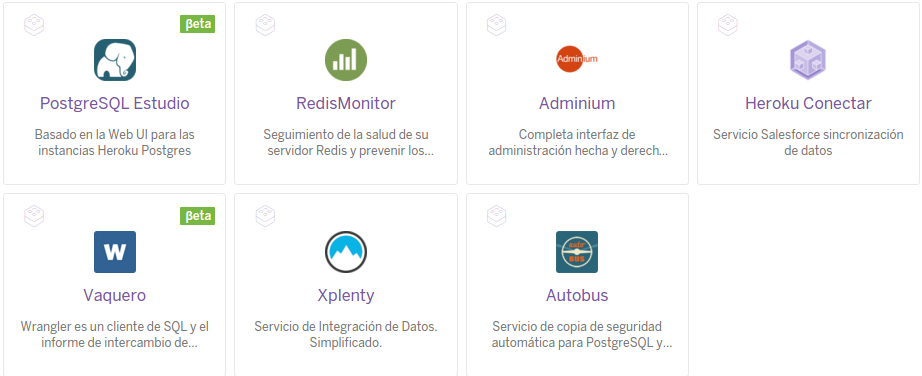
\includegraphics[width=10cm, height=5cm]{ampliacion/3.png}
\end{frame}

\begin{frame}
\frametitle{Heroku. Servicios}
EMAIL/SMS.\\
Incorporar y hacer un seguimiento de mensajería segura y fiable a los usuarios o dentro de su propia aplicación.\\ \ \\
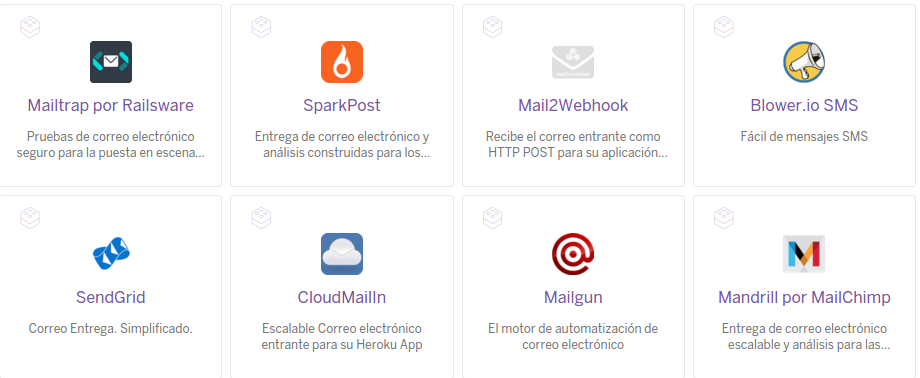
\includegraphics[width=10cm, height=5cm]{ampliacion/4.png}
\end{frame}

\begin{frame}
\frametitle{Heroku. Servicios}
Servicios para ayudarle en pruebas de rendimiento y la calidad de sus aplicaciones.\\ \ \\
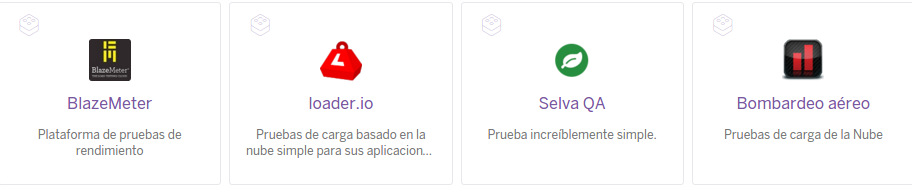
\includegraphics[width=10cm, height=2cm]{ampliacion/5.png}
\end{frame}

\begin{frame}
\frametitle{Heroku. Servicios}
Seguridad.\\ \ \\

\includegraphics[width=10cm, height=2cm]{ampliacion/6.png}
\end{frame}

\begin{frame}
\frametitle{Heroku. Importancia}
La importancia se presenta a la hora de desplegar. Nos brinda una multitud de opciones para elegir desde hostings compartidos a servidores privados, o incluso la famosa nube. Todo dependerá del alcance y necesidades de nuestra aplicación y sobre todo, del presupuesto que tengamos.\\ \ \\
Es una plataforma que nos permite trabajar con aplicaciones web desarrolladas en ruby on rails (y otras tecnologías), también nos permite que concentremos esfuerzos en la creación de aplicaciones y olvidemos de la configuración del servidor.\\
\end{frame}

\begin{frame}
\frametitle{Heroku. Importancia}
Hay que tener en cuenta que un “dynos” es un proceso que atiende a peticiones para las aplicaciones; entre mas dynos hay, mas peticiones atendidas habrá.
En cuanto al tiempo, es óptimo para un proyecto inicial, Heroku podría ayudar a acelerar el tiempo de comercialización del producto en etapas posteriores.\\ \ \\
En cuanto a la prueba de aplicación en Heroku no es obligatorio alcanzar un mínimo en el número de pruebas realizadas. Los nuevos proyectos que duran más de dos meses son desarrollados usando pruebas desde cero.
\end{frame}

\begin{frame}
\frametitle{Heroku. Ventajas}
\begin{itemize}
	\item La mayor ventaja de este paradigma es la rapidez con la que se puede publicar una aplicación a la nube.
	\item Con un comando “git push heroku master”, la aplicación está lista para recibir peticiones. No hay que invertir tiempo en configurar servidores, firewalls, ni bases de datos.
	\item Todo esto viene con un coste adicional asociado, pero generalmente para aplicaciones o equipos pequeños realmente vale la pena ya que ahorra muchos problemas y dolores de cabeza que pueden presentarse si además hay que mantener la infraestructura.
\end{itemize}
\end{frame}

\begin{frame}
\frametitle{Heroku. Desventajas}
\begin{itemize}
	\item La mayor desventaja con servicios como Heroku es la falta de personalización y optimizaciones que pueden realizarse cuando hay acceso más abierto a la infraestructura.
	\item Para una aplicación pequeña esto no es un problema representativo, pero para una aplicación con decenas de millones de visitas al día, las optimizaciones a nivel de infraestructura pueden representar la diferencia entre funcionar o colapsar, además de representar grandes ahorros de coste.
	\item Entre algunas de las alternativas a Heroku encontramos a Google App Engine, Openshift, AppFog y DotCloud.
\end{itemize}
\end{frame}

\begin{frame}
\frametitle{Heroku. Arquitectura}
\centering WebSocket\\ \ \\
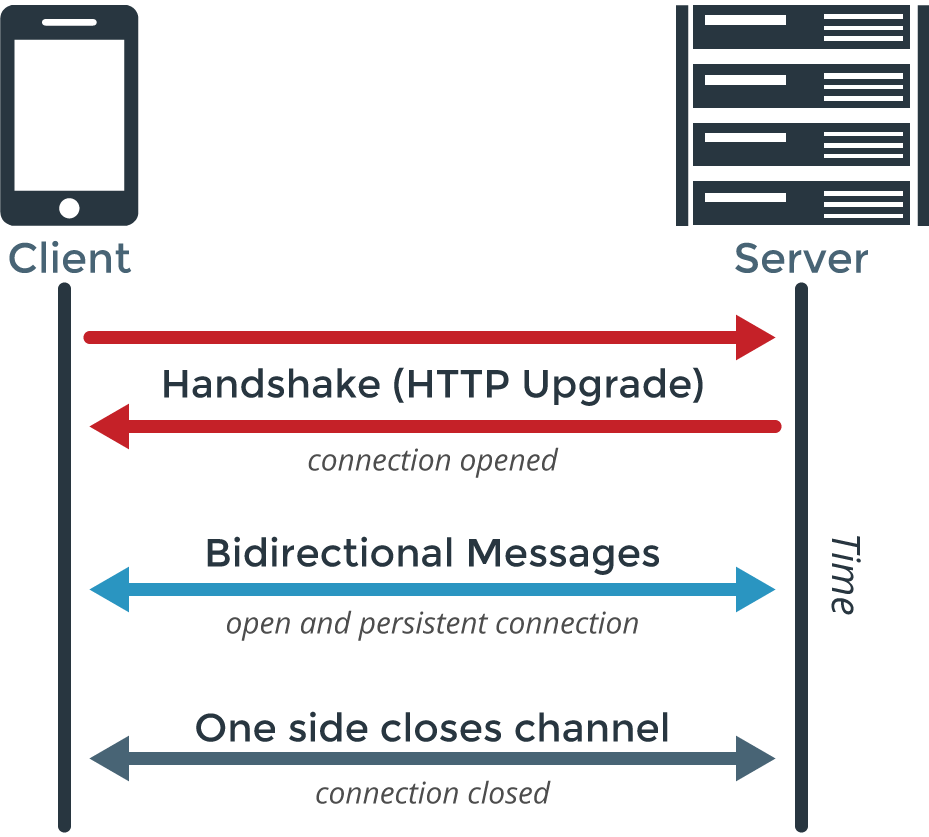
\includegraphics[width=10cm,height=5cm]{arquitectura/1.png}

\end{frame}

\begin{frame}
	\frametitle{Heroku. Arquitectura}
	\centering WebSocket\\ \ \\
	\begin{itemize}
		\item El protocolo WebSocket es una tecnología que forma la base de aplicaciones web modernas en tiempo real.
		\item Proporciona un canal bidireccional para la entrega de datos entre clientes y servidores.
		\item Da la flexibilidad de una conexión TCP con el modelo de seguridad adicional y metadatos incorporados en el protocolo HTTP.
	\end{itemize}
\end{frame}


\begin{frame}
\frametitle{Heroku. Arquitectura}
\centering Tiempo de respuesta HTTP\\ \ \\
\flushleft Cuando una conexión dyno se haya establecido
\begin{itemize}
	\item Las solicitudes HTTP tienen una ventaja de 30 segundos iniciales para que el proceso web devuelva datos de respuesta (ya sea la respuesta completado o una cierta cantidad de datos que eindiqque que el proceso esta activo). 
	\item Los procesos que no envían los datos de respuesta dentro de la ventaja inicial de 30 segundos verán un error.
\end{itemize}
\end{frame}

\begin{frame}
	\frametitle{Heroku. Arquitectura}
	\centering El modelo de Proceso\\ \ \\
\begin{itemize}
	\item Es una abstracción sencilla y potente para ejecutar programas de servidor. 
	\item Aplicado a las aplicaciones web, el modelo de proceso nos da una manera única de pensar en dividir nuestras cargas de trabajo y la ampliación en el tiempo.
	\item El modelo de procesos se utiliza para los dynos web, trabajadores y todos los otros tipos de dinamómetros.
\end{itemize}
\end{frame}

\begin{frame}
	\frametitle{Heroku. Arquitectura}
	\centering Tipos de procesos vs dinamómetros\\ \ \\
	\begin{itemize}
		\item Es un tipo de proceso que realiza prototipo de la que se instancian uno o más dinamómetros.
		\item Esto es similar a la forma en que una clase es el prototipo de la cual se instancian uno o más objetos en la programación orientada a objetos.\\
	\end{itemize}
\end{frame}

\begin{frame}
	\frametitle{Heroku. Arquitectura}
	\centering Tipos de procesos vs dinamómetros\\ \ \\
	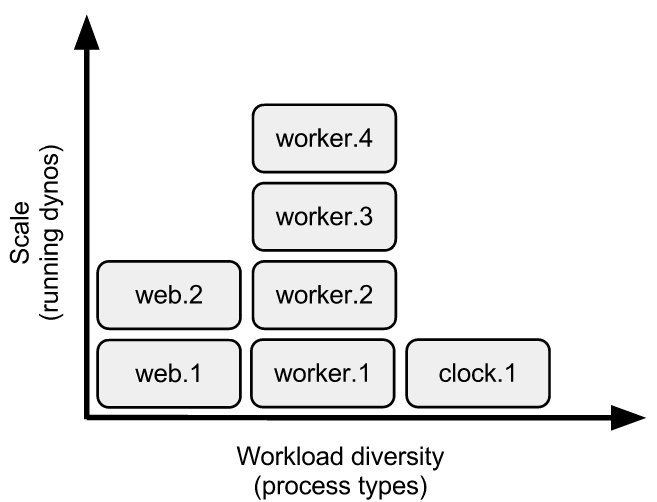
\includegraphics[width=10cm,height=5cm]{arquitectura/tipodeproceso.jpg}
\end{frame}

\begin{frame}
		\frametitle{Heroku. Arquitectura}
	\centering Slug\\ \ \\
	\begin{itemize}
		\item Son comprimidos y copias preenvasadas de su aplicacion optimisados para la distribucion al dyno manager.
		\item Cuando git push a Heroku, su código es recibido por el compilador babosa que transforma su repositorio en una babosa. Escalar una aplicación a continuación descargas y amplía la babosa a un banco de pruebas para su ejecución.
	\end{itemize}
\end{frame}

\begin{frame}
		\frametitle{Heroku. Arquitectura}
	\centering Dynos\\ \ \\
	El compilador Slug es invocado por un git pre-recepción de gancho, que sigue estos pasos:
	\begin{itemize}
		\item Crear una copia nueva de la cabeza de la rama principal. 
		\item Quite cualquier cosa especificada en un archivo .slugignore de nivel superior. 
		\item Descarga, construir e instalar las dependencias locales como se especifica en el archivo de generación (por ejemplo, Gemfile, package.json, requirements.txt, pom.xml, etc.) con la herramienta de gestión de la dependencia con el apoyo del idioma (por ejemplo Bundler, npm, pip, Maven). 
		\item Empaquete el archivo slug final.
	\end{itemize}
\end{frame}

\begin{frame}
		\frametitle{Heroku. Arquitectura}
	\centering Tamaño Slug\\ \ \\

	\begin{itemize}
		\item El tamaño máximo permitido slug (después de la compresión) es de 300 MB. 
		\end{itemize}
	\end{frame}

\begin{frame}
		\frametitle{Heroku. Arquitectura}
	\centering Dynos\\ \ \\
	\begin{itemize}
		\item Un banco de pruebas(Dynos) es un contenedor ligero Linux que ejecuta un único comando especificado por el usuario.
		\item  Un banco de pruebas puede ejecutar cualquier comando disponible en su entorno por defecto (lo que la oferta el Cedar stack) o en su aplicación slug (una copia comprimida y pre-envasados de su aplicacion y sus dependencias)
	\end{itemize}
\end{frame}

\begin{frame}
	\frametitle{Heroku. Arquitectura}
	\centering Tipos de Dynos\\ \ \\
	Heroku corre dinamómetros de tres maneras diferentes: 
	\begin{itemize}
		\item Dynos Web
		\item Dynos Trabajadores
		\item Dynos on-off
	\end{itemize}
\end{frame}
\begin{frame}
	\frametitle{Heroku. Arquitectura}
	\centering Dynos Web\\ \ \\
	\begin{itemize}
		\item Los Dynos Web son dinamómetros de la "web" su tipo de proceso se define en su Procfile. Solamente los dinamómetros web reciben tráfico HTTP desde los routers de Heroku. 
	\end{itemize}
	
\end{frame}
\begin{frame}
	\frametitle{Heroku. Arquitectura}
	\centering Dynos Trabajadores\\ \ \\
	\begin{itemize}
		\item Puede hacer cualquier tipo de proceso que este declarado en su Procfile, distinto de "web". 
		\item Los Dynos trabajadores se utilizan normalmente para trabajos en segundo plano, sistemas de colas y los trabajos programados. 
		\item Puede tener varios tipos de Dynos trabajadores en la aplicación. Por ejemplo, uno para los trabajos urgentes y otra para trabajos de larga duración.
	\end{itemize}
\end{frame}
\begin{frame}
	\frametitle{Heroku. Arquitectura}
	\centering Dynos One-Off \\ \ \\
	\begin{itemize}
		\item Los Dynos Ono-Off son dinamómetros temporales que se pueden ejecutar unifamiliares, o con su entrada / salida conectado a su terminal local.
		\item Están cargados con su último lanzamiento. Pueden ser utilizados para manejar las tareas administrativas, como las migraciones de bases de datos y sesiones de consola. 
		\item También pueden ser utilizadas para ejecutar ocasionalmente trabajo de fondo, con el Programador de Heroku.  
	\end{itemize}
\end{frame}

\begin{frame}
	\frametitle{Heroku. Arquitectura}
	\centering Tipos de Dynos\\ \ \\
	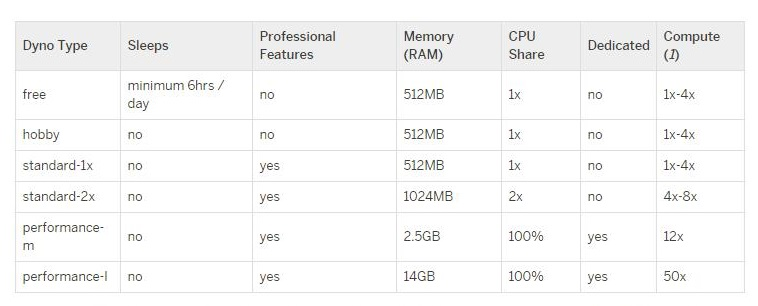
\includegraphics[width=10cm,height=5cm]{arquitectura/dynos.jpg}
	
\end{frame}
\begin{frame}
	\frametitle{Heroku. Arquitectura}
	\centering Tamaño de los Dynos\\ \ \\
	\begin{itemize}
		\item Heroku acredita automáticamente cada aplicación con 750 dyno-hora gratuitas al mes, que están claramente identificados en su factura.
		\item Esta asignación se puede utilizar para cualquier tipo de banco de pruebas de cualquier tamaño del banco de pruebas.
		\item Tenga en cuenta que 2X dinamómetros consumen el doble de Dyno-horas libres comparado con las 750 dyno-hora 1X dynos, 2x se ejecutará de forma gratuita durante 375 horas. 
		\item PX consumen 16 veces más Dyno-horas libres por horas como 1X dinamómetros. 
	\end{itemize}
	
	
\end{frame}
\begin{frame}
	\frametitle{Heroku. Arquitectura}
	\centering Tamaño de Dynos\\ \ \\
	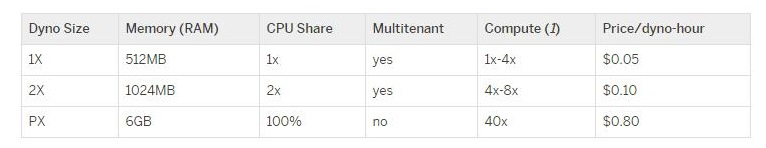
\includegraphics[width=10cm,height=5cm]{arquitectura/dynoshora.jpg}
	
\end{frame}

\begin{frame}
\frametitle{Heroku. Arquitectura}
\centering Dyno Sleeping y App de Recharging\\ \ \\
\begin{itemize}
	\item Las Aplicaciones que utilizan el tipo de banco de pruebas libres tienen un sleeping(sueño) y un comportamiento de recarga.
	\item  Los Dinamómetros gratis dormiran cuando un banco de pruebas no recibe ningún tráfico web por un período de tiempo.
	\item  Si un banco de pruebas libre supera una cuota de 18 horas de actividad durante una ventana de 24 horas, se verá obligada a recargar.
\end{itemize}
\end{frame}

\begin{frame}
\frametitle{Heroku. Arquitectura}
\centering Dyno Sleeping y App de Recharging\\ \ \\
Una aplicación está activa si alguna parte de la aplicación se está ejecutando. Por ejemplo, si algunos de las siguientes condiciones son verdaderas:
\begin{itemize}
\item Hay un banco de pruebas web que está recibiendo tráfico.
\item Hay un banco de pruebas trabajador que se está ejecutando. 
\item Un banco de pruebas on-off esta corriendo. Por ejemplo, se inició a través de la CLI o el planificador.
\end{itemize}
\end{frame}


\begin{frame}
	\frametitle{Heroku. Arquitectura}
	\centering Sleeping\\ \ \\
	\begin{itemize}
		\item Si una aplicación tiene un Dyno web y no recibe ningún tráfico en un período de 30 minutos, el Dyno web va a dormir.
		\item Además de dormir el dyno web, el Dyno trabajador (si está presente) también va a dormir. 
		\item Si un Dyno web recibe tráfico, se activará de nuevo después de un breve retraso. 
		\item Si la aplicación tiene Dyno trabajador que fue a dormir antes de ampliase, será ampliado de nuevo también.
	\end{itemize}
\end{frame}

\begin{frame}
	\frametitle{Heroku. Arquitectura}
	\centering Recharging\\ \ \\
	\begin{itemize}
		\item Las aplicaciones en el estado "recarga" se cierran durante 6 horas. 
		\item Si un Dyno (ya sea web, trabajador o one-off) se ejecutarán durante este período de tiempo.Cualquier tráfico web recibida en este estado devolverá una página de error.
	\end{itemize}
\end{frame}

\begin{frame}
\frametitle{Heroku. Registro}
Para el registro en Heroku solo debemos rellenar el siguiente formulario.\\ \ \\
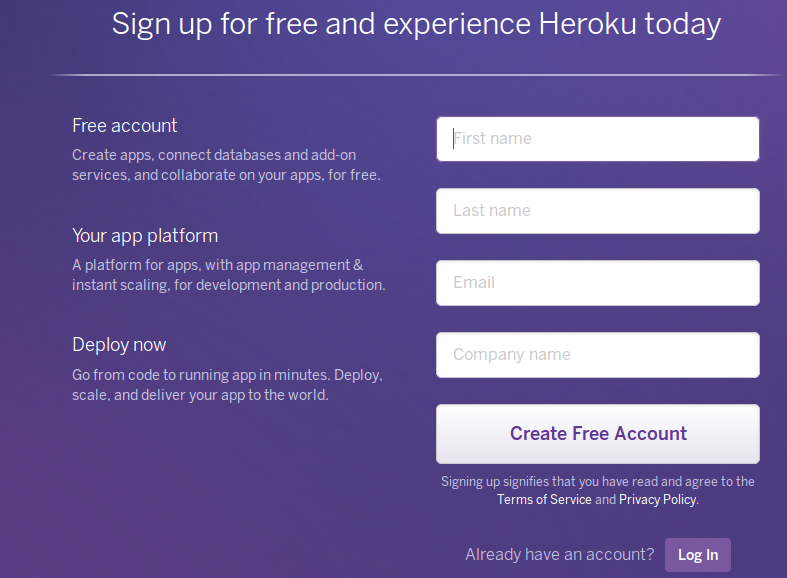
\includegraphics[width=10cm, height=5cm]{githubHeroku/22.png}
\end{frame}

\begin{frame}
\frametitle{Heroku. Heroku Toolbelt}
Es una herramienta de línea de comandos para trabajar con la plataforma Heroku en OS X, Windows y Debian/Ubuntu. Para la instalación debemos dirigirnos al siguiente enlace \href{https://toolbelt.heroku.com}{LINK}. Seleccionar nuestro sistema operativo y seguir el procedimiento correspondiente.
\end{frame}

\begin{frame}
\frametitle{Heroku. Heroku Toolbelt}
En este caso usaremos Ubuntu. Por lo que ejecutaremos en consola el comando de la imagen.\\ \ \\
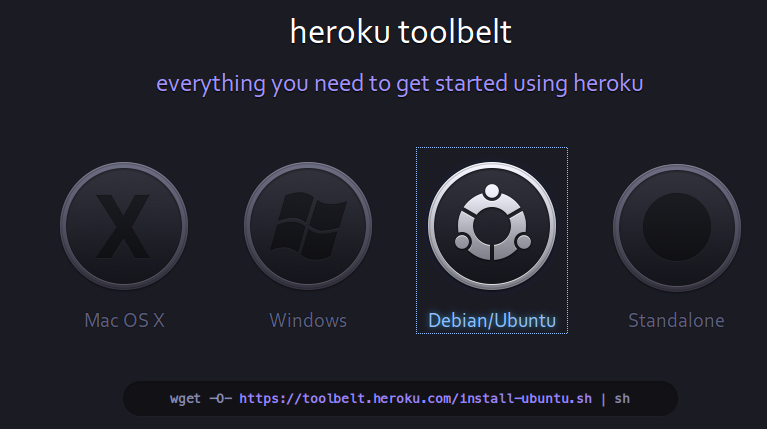
\includegraphics[width=10cm, height=5cm]{githubHeroku/23.png}
\end{frame}

\begin{frame}
\frametitle{Heroku. Heroku Toolbelt}
Una vez instalado debemos loggearnos. Para ello en una terminal escribimos \textit{heroku login}. Nos pedirá el email con el que nos registramos y nuestra contraseña. Una vez hecho esto ya podemos desplegar nuestra aplicación en Heroku.\\ \ \\
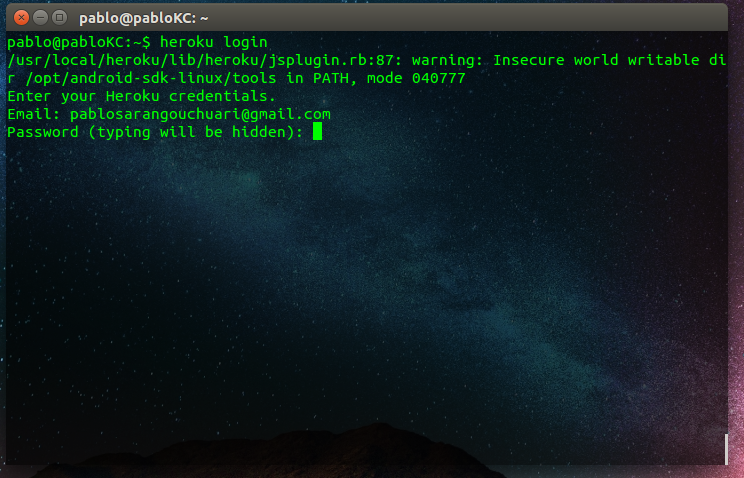
\includegraphics[width=10cm, height=5cm]{githubHeroku/5.png}
\end{frame}

\begin{frame}
\frametitle{Despliegue. GitHub}
A partir de un proyecto existente en GitHub haremos el despliegue en Heroku.\\ \ \\
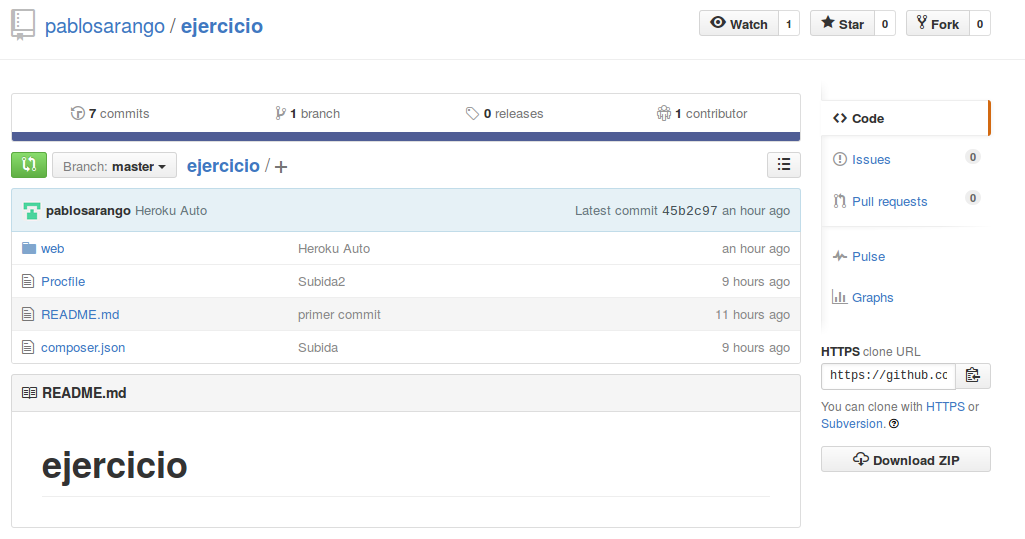
\includegraphics[width=10cm, height=5cm]{githubHeroku/24.png}
\end{frame}

\begin{frame}
\frametitle{Despliegue. Requisitos}
Para este ejemplo usaremos una aplicación sencilla en PHP. Para que Heroku reconozca que nuestra aplicación está en PHP debemos definir en la raíz de nuestro proyecto un archivo llamado \textit{composer.json}. Una opción es instalar \textit{Composer}, el cual es un gestor de dependencias para PHP. Dada la sencillez de nuestro aplicativo no usaremos dependencias por lo que no es necesario la instalación del gestor. No obstante si es necesario la existencia del archivo \textit{composer.json}.\\ \ \\
Dependiendo del lenguaje de nuestra aplicación deberemos seguir unos u otros pasos para que Heroku sea capaz de ejecutarla. Esta información la podemos encontrar en la página oficial de Heroku.
\end{frame}

\begin{frame}
\frametitle{Despliegue. Requisitos}
La estructura de nuestro archivo \textit{composer.json} es la siguiente.\\ \ \\
\centering
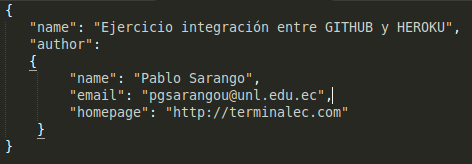
\includegraphics[width=8cm, height=4cm]{githubHeroku/26.png}
\end{frame}

\begin{frame}
\frametitle{Despliegue. Requisitos}
Además del archivo \textit{composer.json} es necesario crear un archivo llamado \textit{Procfile} el cual nos permitirá tener acceso a nuestra aplicación en Heroku. Este archivo no tiene extensión. El contenido de este archivo variará según el tipo de aplicación que estemos corriendo. Tener en cuenta que nosotros tenemos nuestro código php en una carpeta llamada "web". Razón por la cual especificamos esto en nuestro archivo Procfile\\ \ \\
\centering
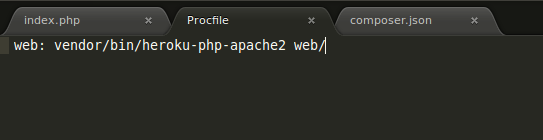
\includegraphics[width=10cm, height=3cm]{githubHeroku/32.png}
\end{frame}

\begin{frame}
\frametitle{Despliegue. Heroku}
En una terminal y posicionados en el directorio de nuestro proyecto ejecutamos el siguiente comando \textit{heroku create}. Ahora ya tenemos la dirección url de nuestro proyecto así como un repositorio remoto de nuestra aplicación en Heroku. Heroku establecerá un nombre aleatorio a nuestro proyecto.\\ \ \\
\centering
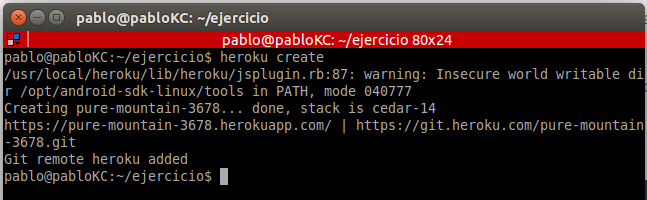
\includegraphics[width=8cm, height=4cm]{githubHeroku/14.png}
\end{frame}

\begin{frame}
\frametitle{Despliegue. Heroku}
Ahora procedemos a subir el código fuente de nuestra aplicación con el comando \textit{git push heroku master}.\\ \ \\
\centering
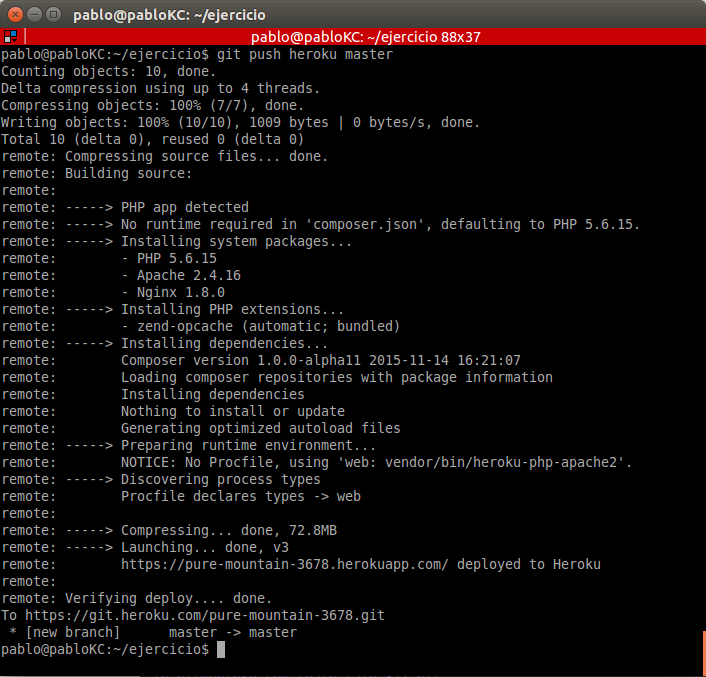
\includegraphics[width=10cm, height=6cm]{githubHeroku/19.png}
\end{frame}

\begin{frame}
\frametitle{Despliegue. Heroku}
Ahora nuestra aplicación ya se encuentra corriendo en Heroku. Para acceder a ella podemos ingresar a la url que vimos anteriormente o podemos ejecutar en consola el comando \textit{heroku open}.\\ \ \\
\centering
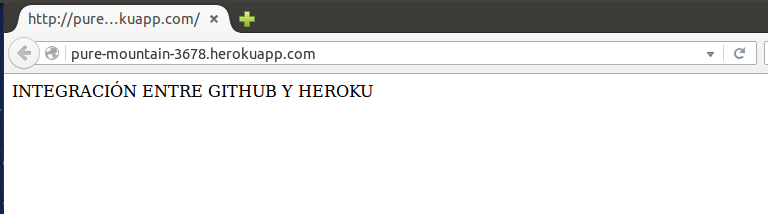
\includegraphics[width=10cm, height=4cm]{githubHeroku/27.png}
\end{frame}

\begin{frame}
\frametitle{GitHub y Heroku. Sincronización}
Lo siguiente es entrar a nuestra cuenta de Heroku y seleccionar nuestra aplicación. Para la sincronización debemos irnos a la sección \textit{Deploy} y acceder al tab de \textit{GitHub}. Posteriormente debemos buscar nuestro repositorio y conectarlo.\\
\centering
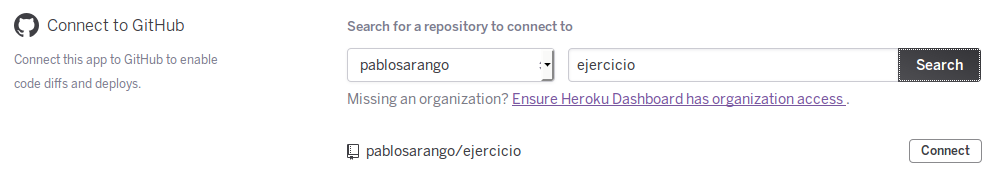
\includegraphics[width=10cm, height=2cm]{githubHeroku/15.png}
\\ \ \\

\includegraphics[width=10cm, height=2cm]{githubHeroku/16.png}
\end{frame}

\begin{frame}
\frametitle{GitHub y Heroku. Commit}
Cuando hayamos realizado cambios a nuestro código y queremos que estos se vean reflejados en nuestra aplicación en Heroku debemos hacer \textit{commit} a GitHub y actualizar en Heroku. Para ello escribimos los comandos de la imagen. Se nos pedirá nuestro usuario de GitHub y contraseña.\\
\centering
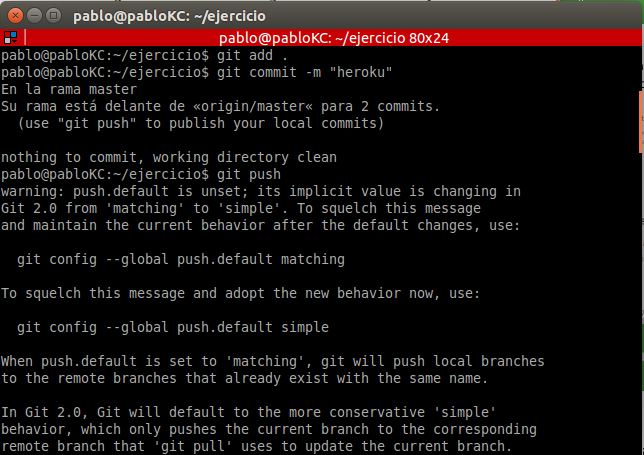
\includegraphics[width=10cm, height=5cm]{githubHeroku/28.png}
\end{frame}

\begin{frame}
\frametitle{GitHub y Heroku. Despliegue Automático}
Para reflejar los cambios de manera automática en Heroku nos dirigimos a nuestra aplicación, después a la sección \textit{Deploy} y al tab \textit{GitHub}. Ahí tendremos que activar el despligue automático.\\ \ \\
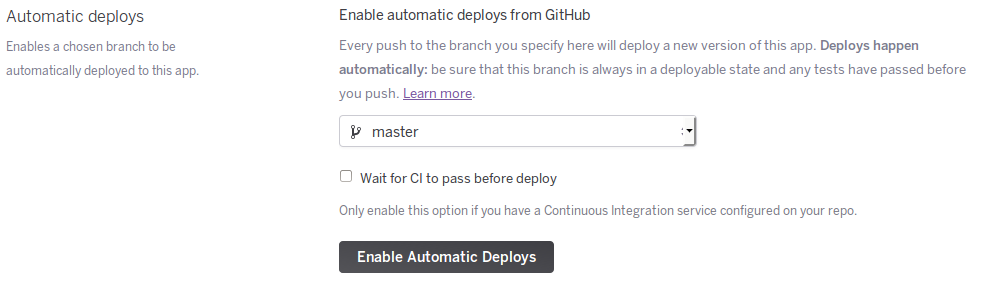
\includegraphics[width=10cm, height=5cm]{githubHeroku/33.png}
\end{frame}

\begin{frame}
\frametitle{GitHub y Heroku. Despliegue Automático}
Con esto cada vez que hagamos \textit{push} nuestra aplicación se actualizará en Heroku automáticamente. \\ \ \\
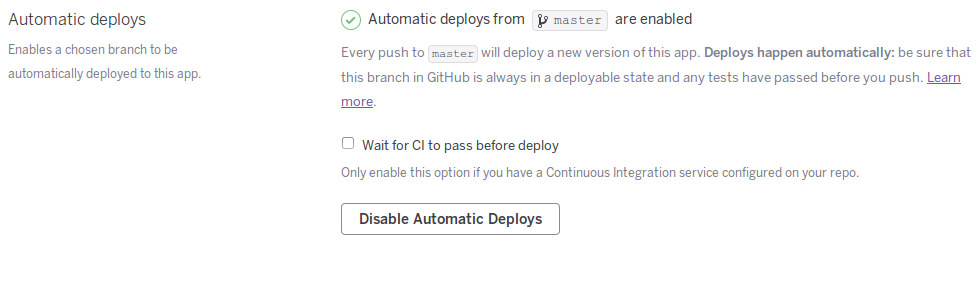
\includegraphics[width=10cm, height=5cm]{githubHeroku/34.png}
\end{frame}

\begin{frame}
\frametitle{GitHub y Heroku. Despliegue Manual}
En nuestra aplicación nos vamos a la sección \textit{Deploy} y al tab de \textit{GitHub}. Al final de la página encontraremos una sección que la que haciendo click en \textit{Deploy Branch} se reflejarán los cambios que hemos hecho a nuestra aplicación.\\
\centering
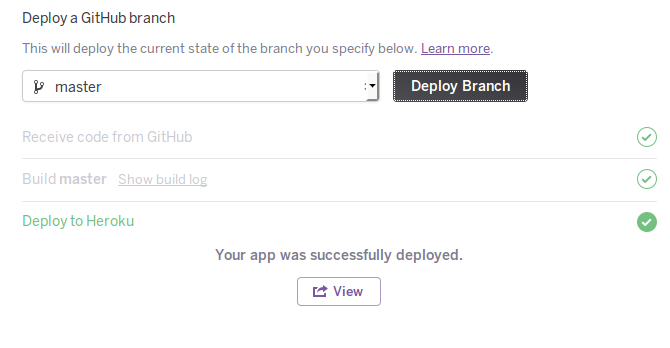
\includegraphics[width=10cm, height=5cm]{githubHeroku/30.png}
\end{frame}

\begin{frame}
\frametitle{GitHub y Heroku. Commit}
Ahora ya estarán disponibles los cambios en nuestra aplicación.\\ \ \\
\centering
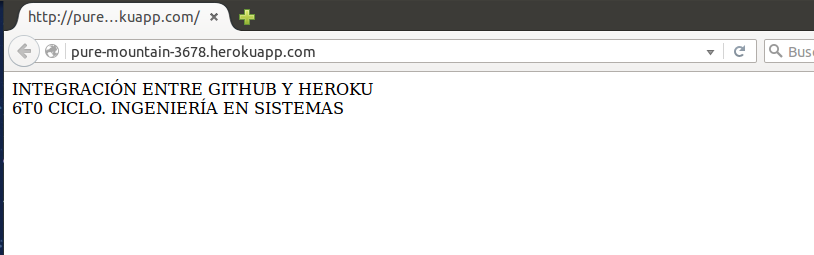
\includegraphics[width=10cm, height=5cm]{githubHeroku/31.png}
\end{frame}

\subsection{Conclusiones}
\begin{frame}
\frametitle{Conclusiones}
El empleo de una Plataforma como Servicio, en este caso Heroku, permite a los desarrolladores abandonar el uso de servidores para sus aplicaciones. Este tipo de servicio les ofrece un gran abanico posibilidades. La mayoría posibilitan usarlos de manera gratuita con aplicaciones pequeñas, además, brinda la oportunidad de pagar cuando la aplicación esté terminada. Dependiendo de la escalabilidad de la aplicación estos servicios proporcionan la capacidad de comprar nuevas características y en algunos casos pagar solo por el tiempo que se use más requerimientos.

\end{frame}

\begin{frame}
\frametitle{Conclusiones}
Permite enfocarse en el desarrollo de la aplicación al no tener que preocuparse por la configuración de servidores y la implementación de estos. Otra ventaja es que el despliegue se hace a través de Git. Por lo que si trabajamos con Git nos resultará fácil adaptarnos al funcionamiento de Heroku. Heroku también detecta automáticamente qué tipo de aplicación estamos subiendo, así, si detecta que es una aplicación en Ruby on Rails lanzará rails server, o python app/manage.py si estamos usando DJango.
\end{frame}


\subsection{Bibliografía}
\begin{frame}
\frametitle{Bibliografia}
\bibliographystyle{IEEEannot}
\bibliography{biblio}
\end{frame}

\subsection{Licencia}
\begin{frame}
\frametitle{Licencia}
\begin{center}
\href{http://creativecommons.org/licenses/by-nc/4.0/}{
\includegraphics[scale=.8]{cc}}
\end{center}
\end{frame}

\MuchasGraciasFrame

\end{document}